\documentclass[xcolor={svgnames},
  %hyperref={colorlinks,citecolor=Blue,linkcolor=Blue,urlcolor=DarkBlue}, 
  hyperref={colorlinks},
  %handout,
  t,
  spanish, 12pt]{beamer}
  \mode<presentation>
  
  \usefonttheme[onlymath]{serif}
  \setbeamertemplate{theorems}[ams style] 
  
  \addtolength{\headsep}{1cm}
  
\usetheme{metropolis}
 \useinnertheme{rectangles} %\setbeamertemplate{navigation symbols}{}
%\setbeamertemplate{caption}[numbered]
%\useoutertheme{infolines}
%\usepackage{cleveref}

\metroset{block=fill}
%\usecolortheme{beaver}
\usecolortheme{dolphin}
%\usecolortheme{whale}

\setbeamercovered{highly dynamic}

\newcounter{saveenumi}
\newcommand{\seti}{\setcounter{saveenumi}{\value{enumi}}}
\newcommand{\conti}{\setcounter{enumi}{\value{saveenumi}}}

\resetcounteronoverlays{saveenumi}

%\pagestyle{empty}
\setbeamercolor{emph}{fg=purple}
\renewcommand<>{\emph}[1]{%
  {\usebeamercolor[fg]{emph}\only#2{\itshape}#1}%
}

%\usepackage{beamerthemebars}
\usepackage{fontenc}
\usepackage{graphicx}
\usepackage[utf8]{inputenc}
\usepackage[spanish,mexico]{babel}
\usepackage{fontenc}
\usepackage{amsmath}
\usepackage{amsthm}
\usepackage{amssymb}
\usepackage{graphicx}
\usepackage{mathrsfs}
\usepackage{yfonts}
%\usepackage{hyperref}
\usepackage{enumerate}
\usepackage{mathtools}
\usepackage{textcomp}
\usepackage{lmodern}
\usepackage{fancyvrb}
\usepackage{multicol}
\usepackage{color}
\usepackage{verbatim}

\DefineVerbatimEnvironment{ColorVerbatim}{Verbatim}%
  {formatcom=\color{purple},commandchars=\\\{\}}
  
\usepackage{etoolbox}

\BeforeBeginEnvironment{Verbatim}{\begingroup\color{purple}}%
\AfterEndEnvironment{Verbatim}{\endgroup}%
%\usepackage{etoolbox}
% \AtBeginEnvironment{enumerate}{\begin{multicols}{2}}    %%% this line
% \AtEndEnvironment{enumerate}{\end{multicols}}            %%% and this one
% \usepackage{multicol}
%\usepackage[usenames,dvipsnames,svgnames,table]{xcolor}
%\usepackage[urlcolor=blue]{hyperref}
%\numberwithin{section}{part}
\numberwithin{equation}{section} %% Comment out for sequentially-numbered
\numberwithin{figure}{section} %% Comment out for sequentially-numbered

% Automatically generate section title slides in beamer?
% Add support for \subsubsectionpage
\def\subsubsectionname{\translate{}}
\def\insertsubsubsectionnumber{\arabic{subsubsection}}
\setbeamertemplate{subsubsection page}
{
  \begin{centering}
    {\usebeamerfont{subsubsection name}\usebeamercolor[fg]{subsubsection name}\subsubsectionname}%~\insertsubsubsectionnumber}
    \vskip1em\par
    \begin{beamercolorbox}[sep=4pt,center]{part title}
      \usebeamerfont{subsubsection title}\insertsubsubsection\par
    \end{beamercolorbox}
  \end{centering}
}
\def\subsubsectionpage{\usebeamertemplate*{subsubsection page}}

\AtBeginSection{\frame{\sectionpage}}
\AtBeginSubsection{\frame{\subsectionpage}}
\AtBeginSubsubsection{\frame{\subsubsectionpage}}

\theoremstyle{plain}
  \newtheorem{thm}{Teorema}[section]
  \newtheorem{prop}{Proposici\'on}[section]
  \newtheorem{lem}[thm]{Lema}
  \newtheorem{cor}[thm]{Corolario}
  %\newtheorem{rem}{Observaci\'on}[chapter]
  \newtheorem*{sol}{Soluci\'on}
  \newtheorem{alg}{Algoritmo}[section]
  \newtheorem{solved}{Ejercicio Resuelto}
  \newtheorem{evc}{Evaluaci\'on Continua}

\theoremstyle{definition}
  \newtheorem{defn}{Definici\'on}[section]
  \newtheorem{conj}{Conjectura}[section]
  \newtheorem{exmp}{Ejemplo}[section]
  \newtheorem{exe}{Evaluaci\'on Continua}[section]
  \newtheorem{prob}{Problema}[section]
  \newtheorem{rem}{Observaci\'on}[section]
  \newtheorem*{ax}{Axioma}
  \newtheorem{tdv}{Tabla de Verdad}

\theoremstyle{remark}
  \newtheorem{claim}{Afirmaci\'on}[section]
  %\newtheorem{rem}{Observaci\'on}[chapter]
  %\newtheorem*{note}{Nota}
  \newtheorem{case}{Caso}
  \newtheorem{hint}{Sugerencia}[section]


\numberwithin{equation}{section}
\newcommand{\p}{\partial}
%\newcommand{\T}{\mathbb{T}}
\newcommand{\R}{\mathbb{R}}
\newcommand{\N}{\mathbb{N}}
\newcommand{\Q}{\mathbb{Q}}
\newcommand{\abs}[1]{\left|#1\right|}
\newcommand{\f}{\phi}
\newcommand{\vphi}{\varphi}
\newcommand{\vf}{\varphi}
\newcommand{\flow}[2]{\varphi^{#1}\left( #2 \right)}
\renewcommand{\d}[1]{\dot{#1}}
\renewcommand{\r}{\rho}
\newcommand{\A}{\mathcal{A}}
\newcommand{\gam}{\gamma}
\newcommand{\lam}{\lambda}
\renewcommand{\a}{\alpha}
\renewcommand{\b}{\beta}
\newcommand{\om}{\omega}
\newcommand{\iso}{\simeq}
\newcommand{\tensor}{\otimes}
\newcommand{\Z}{\mathbb{Z}}
\newcommand{\set}[1]{\left\{ #1 \right\}}
\newcommand{\inc}{\hookrightarrow}
\renewcommand{\L}{\mathcal{L}}
\renewcommand{\H}{\mathcal{H}}
\newcommand{\D}{\mathcal{D}}
\newcommand{\converge}[1]{\xrightarrow{#1}}
\renewcommand{\cot}{T^{*}}
\newcommand{\cott}[1]{T^{*}\T^{#1}}
\newcommand{\ep}{\epsilon}
\newcommand{\inp}[1]{\langle #1 \rangle}
%\newcommand{\G}{\mathcal{G}}
\newcommand{\hu}{\textbf{h}}
\newcommand{\deck}[1]{\operatorname{Dake}\left( #1 \right)}
\newcommand{\til}[1]{\tilde{#1}}
\newcommand{\Gam}{\Gamma}
\newcommand{\grad}{\nabla}
\newcommand{\del}{\delta}
\newcommand{\id}{\operatorname{Id}}
\newcommand{\Del}{\Delta}
\newcommand{\var}{\Delta}
\newcommand{\avch}[2]{\frac{\Delta #1}{\Delta #2}}
\newcommand{\Avch}[2]{\dfrac{\Delta #1}{\Delta #2}}
\newcommand{\Err}{\operatorname{Err}}
\newcommand{\imply}{\rightarrow}
\newcommand{\wed}{\wedge}
\newcommand{\biconditional}{\longleftrightarrow}
\newcommand{\yields}{\vdash}
\newcommand{\onlyif}{\Rightarrow}
\newcommand{\uset}{\mathbb{U}}
\newcommand{\minus}{\backslash}
\newcommand{\symdif}{\oplus}
\newcommand{\rel}[1]{\boxed{{\color{blue}\textbf{#1}}}}
\newcommand{\dom}[1]{\operatorname{Dom}\left( #1 \right)}
\newcommand{\im}[1]{\operatorname{Im}\left( #1 \right)}
\newcommand{\nrel}[1]{\boxed{{\color{red}\not}{\color{orange}\textbf{#1}}}}
\newcommand{\comp}[2]{#1 \circ #2}

%\date{\today}
\title{Matem\'aticas Discretas \\
Relaciones y funciones}
\author[Juliho Castillo]{\href{https://www.youtube.com/channel/UCb1i-EtybaWWX5urFfmMUWQ}{M. en C. Juliho Castillo}}

\institute[ITESM-CCM]{Tec de Monterrey, Campus Ciudad de M\'exico}
\date{\today}

\begin{document}

\logo{
 
\includegraphics[width=1cm,keepaspectratio=true]{./logo.png}
 %LOGO-CECYTEO.png: 200x200 pixel, 72dpi, 7.06x7.06 cm, bb=0 0 200 200
}

\frame{
\titlepage
}

\begin{frame}[allowframebreaks=0.5]
 \tableofcontents
\end{frame}

%\frame{\tableofcontents}

% \AtBeginSubsection[]
% {
%   \begin{frame}
%     \tableofcontents[currentsubsection]
%   \end{frame}
% }

\section{Relaciones}

\begin{frame}
\frametitle{Ejemplos de relaciones}
\begin{itemize}
 \item ``menor que''
 \item ``es paralelo a''
 \item ``es un subconjunto de''
\end{itemize}

\end{frame}

\begin{frame}
Formalmente, definiremos una relaci\'on en t\'erminos de \emph{pares ordenados.}
\end{frame}

\begin{frame}
\begin{defn}
 Un \emph{par ordenado} de elementos $a$ y $b,$ donde $a$ es el primer elemento y $b$ es el segundo se denota por $(a,b).$
\end{defn}

\end{frame}

\begin{frame}

\begin{ax}
 $(a,b)=(c,d)$  si y s\'olo si $a=c$ y
$b=d.$
\end{ax}

\pause

En particular $(a,b)\neq(b,a),$  al menos que $a=b.$

\pause

Esto es muy diferente al caso de un conjunto, d\'onde el orden es irrelevante:
$$
\set{a,b}=\set{b,a}.
$$
\end{frame}

\subsection{Producto de conjuntos}

\begin{frame}
Consideremos dos conjuntos arbitrarios $A$ y $B.$ El conjunto de todos los pares ordenadors $(a,b)$ donde $a\in A, b \in B$ es llamado \emph{producto(cartesiano)} de $A$ con $B,$ y se denota por $A \times B,$ es decir,
$$
A \times B = \set{(a,b) \mid a \in A, \; b \in B}
$$
\end{frame}

\begin{frame}
Podemos construir el producto cartesiano de un conjunto $A$ consigo mismo, y en ese caso denotaremos
$$A^{2}= A\times A.$$
\end{frame}

\begin{frame}
\begin{exmp}
 Sea $A=\set{x,y}, \, B={0,1}.$ Entonces
 \begin{enumerate}
  \item $A^{2}=\set{(x,x), (x,y), (y,x), (y,y)}$
  \item $A\times B= \set{(x,0), (x,1), (y,0), (y,1)}$
  \item $B\times A= \set{(0,x), (0,y), (1, x), (1,y)}$
  \item $B^2=\set{(0,0), (0,1), (1,0), (1,1)}$
 \end{enumerate}

\end{exmp}

\end{frame}

\begin{frame}
 \begin{rem}
  \begin{itemize}
   \item En general, $A\times B \neq B \times A.$
   \item Si \emph{$n(A)$} denota el \emph{n\'umero de elementos} en el conjunto $A,$ entonces
   $$
   n(A \times B)= n(A) \cdot n(B).
   $$
  \end{itemize}

 \end{rem}

\end{frame}


\begin{frame}
 Sean $A=\set{1,2}$ y $B={a,b,c}.$ Determine $A\times B,$ $B\times A$ y $A^{2},$ y describa gr\'aficamente estos productos.
\end{frame}

\begin{frame}
\begin{exmp}
 $\R^{2}=\R \times \R$ es llamado frecuentemente el \emph{plano Cartesiano.}
\end{exmp}

\end{frame}

\begin{frame}
\begin{defn}
 Definimos el producto cartesiano de un n\'umero finito de conjuntos $A_{1},...,A_{n}$ como
 $$
 \prod_{i=1}^{n} A_{i}= A_{1} \times \cdots \times A_{n}=\set{\left( a_{1},\dots,a_{n} \right)\mid a_{1}\in A_{1}, \dots, a_{n}\in A_{n}}
 $$
\end{defn}

\end{frame}

\begin{frame}
\begin{rem}
 De manera an\'aloga al caso $n=2,$ definiremos
 $$
 A^{n}=\prod_{i=1}^{n}A.
 $$
 \pause
 
 Por ejemplo, $\R^{3}$ denota el espacio tridimensional.
\end{rem}

\end{frame}

\subsection{Relaciones}

\begin{frame}
\begin{defn}
 Sean $A$ y $B$ conjuntos arbitrarios. Una \emph{relaci\'on binaria $R$,} o simplemente relaci\'on, de $A$ a $B$ es un subconjunto de $A \times B.$
\end{defn}

\end{frame}

\begin{frame}
Para cada $(a,b)\in A \times B$ alguna de las siguientes condiciones (pero no ambas) es cierta:
\begin{enumerate}
 \item $(a,b)\in R;$ en cuyo caso diremos que \emph{$a$ est\'a $R-$relacionado con $b$,} y escribiremos $a \rel{R} b.$
 \item $(a,b)\not\in R;$ en cuyo caso diremos que \emph{$a$ no est\'a $R-$relacionado con $b$,} y escribiremos $a \nrel{R} b.$
\end{enumerate}

\end{frame}

\begin{frame}
Si $R$ es una relaci\'on de $A$ en s\'im mismo, es decir $R \subset A^{2},$ entonces diremos que $R$ es una \emph{relaci\'on en $A$.}
\end{frame}

\begin{frame}
\begin{defn}
 Si $R \subset A \times B$ es una relaci\'on, el \emph{domino de $R$} es 
 $$
 \dom{R}=\set{a\in A\mid (a,b)\in R},
 $$ mientras que la \emph{imagen de $R$} es 
 $$
 \im{R}=\set{b\in B\mid (a,b)\in R}.
 $$
\end{defn}

\end{frame}

\subsection{Ejemplos}
\begin{frame}
Sean $A=\set{1,2,3},$ $B=\subset{x,y,z}$ y $$R=\set{(1,y), (1,z), (3,y)}.$$ Entonce $R$ es una relaci\'on de $A$ en $B,$ porque $R \subset A \times B.$
\pause

Respecto a esta relaci\'on, por ejemplo,
$$
1\rel{R}y, \; 1\rel{R}z, \; 3\rel{R}y,
$$ pero 
$$
1\nrel{R}x, 2\nrel{R}x, 2\nrel{R}y.
$$

\pause
En este caso, $\dom{R}=\set{1,3}$ e $\im{R}=\set{y,z}.$
\end{frame}

\begin{frame}
La propia inclusi\'on $\subset$ es una relaci\'on en una colecci\'on de conjuntos $A_{1},...,A_{n}.$ \pause

Para cualquier par $A_{i}, A_{j}$ en dicha colecci\'on $A \subset B$ o $A \not\subset B.$
\end{frame}

\begin{frame}
Una relaci\'on en el conjunto $\Z$ de n\'umero enteros es \emph{\texttt{``$m$ divide a $n.$''}}
\pause

La notaci\'on convencional para esta relaci\'on es \emph{$m \mid n.$}
\end{frame}

\begin{frame}
Consideremos el conjunto de lineas $L$ en el plano. La perpendicularidad $\perp$ es una relaci\'on en $L.$ \pause De manera similar el paralelismo $\parallel.$
\end{frame}

\begin{frame}
 Sea $A$ cualquier subconjunto. Una relaci\'on importante en $A$ es la \emph{igualdad}
 $$
 \set{(a,a) \mid a \in A}
 $$ que usualmente se denota por \emph{$$``=.''$$} 
 \pause En ocasiones, tambi\'en se le llama \emph{entidad} o \emph{diagonal} y se denota por $\triangle_{A},$ o simplemente por $\triangle.$
\end{frame}

\begin{frame}
Sea $A$ un conjunto arbitrario. Entonces tanto $A\times A$ como $\emptyset$ son subconjuntos de $A \times A,$ y son llamados \emph{relaci\'on universal} y \emph{relaci\'on vac\'ia,} respectivamente.
\end{frame}

\begin{frame}
\frametitle{Relaci\'on inversa}

Sea $R$ una relaci\'on de $A$ en $B.$ La \emph{relaci\'on inversa} de $R,$ denotada por \emph{$R^{-1}$,} es la relaci\'on de $B$ en $A$ que consiste en todos aquellos pares que al invertirlos, pertenecen a $R.$ \pause

En otras palabras
$$
R^{-1}=\set{(b,a)\mid (a,b)\in R}.
$$
\end{frame}

\begin{frame}
\begin{exmp}
 Sea $A=\set{1,2,3}, B=\set{x,y,z}$ y $R=\set{(1,y),(1,z),(3,y)}.$ Entonces
 $$
 R^{-1}=\set{(y,1), (z,1), (y,3)}.
 $$
\end{exmp}
\end{frame}

\begin{frame}
\begin{rem}
 \begin{itemize}
  \item $\left( R^{-1} \right)^{-1}=R.$
  \item $\dom{R^{-1}}=\im{R}$
  \item $\im{R^{-1}}=\dom{R}$
 \end{itemize}
\end{rem}
\end{frame}



\subsection{Composici\'on de Relaciones}
\begin{frame}
 Sean $A,B,C$ conjuntos arbitrarios, $R$ una relaci\'on de $A$ en $B$ y $S$ una relaci\'on de $B$ en $S.$ \pause Entonces podemos definir una nueva relaci\'on de $A$ en $C$ denotada por \emph{$RS$:}
 \begin{center}
  $a\rel{{RS}}c$ si para alguna $b \in B,$ $a\rel{R}b$ y $b\rel{S}c.$
 \end{center} 
\end{frame}

\begin{frame}
Esto es
$$
RS=\set{(a,c)\mid \exists b\in B: (a,b)\in R, (b,c)\in S}
$$
\end{frame}

\begin{frame}
Supongamos que $R$ es una relaci\'on en $A.$ Entonces, definimos $R^{n}$ de manera recursiva
$$
R^{1}=
\begin{cases}
 R & n=1 \\
 R^{n-1}R & n>1
\end{cases}
$$
\end{frame}

\begin{frame}
\begin{exmp}
 Sea $A=\set{1,2,3,4},$ $B=\set{a,b,c,d}$ y $C=\set{x,y,z}$ y definimos las relaciones: 
 $$R=\set{(1,a),(2,d),(3,a),(3,b),(3,d)}$$  $$S=\set{(b,x),(b,z),(c,y),(d,z)}.$$ Encuentre $RS.$
\end{exmp}

\end{frame}

\begin{frame}
\begin{thm}
 Supongamos que $R$ es uan relaci\'on de $A$ en $B,$ y $S$ una relaci\'on de $B$ en $C.$ Entonces
 $$
 (RS)T=R(ST).
 $$
\end{thm}

\end{frame}

\subsection{Tipos de relaciones}

\subsubsection{Relaciones reflexivas}

\begin{frame}

Una relaci\'on $R$ es un conjunto $A$ es \emph{reflexiva} si $a\rel{R}a$ para todo $a\in A$,\pause \, es decir, $\forall a \in A: (a,a)\in \R.$ \pause

Entonces, $R$ es \emph{no-reflexiva} si...
\end{frame}

\begin{frame}
\begin{exmp}
\label{lip:exmp:2.5}
 Sea $A=\set{1,2,3,4}.$ Determine cuales de las siguientes relaciones son reflexivas:
 \begin{itemize}
  \item $R_{1}=\set{(1,1),(1,2),(2,3),(1,3),(4,4)}$ \pause
  \item $R_{2}=\set{(1,1),(1,2),(2,1),(2,2),(3,3),(4,4)}$ \pause
  \item $R_{3}=\set{(1,3),(2,1)}$\pause
  \item $R_{4}=\emptyset$\pause
  \item $R_{5}=A \times A$
 \end{itemize}

\end{exmp}

\end{frame}

\begin{frame}
\begin{exmp}
 \label{lip:exmp:2.6}
 Determine cuales de las siguientes relaciones son reflexivas:
\begin{itemize}
 \item $\leq$ en $\Z$ \pause
 \item $\subset$ en $2^{A}$ \pause
 Aquí $A$ es un conjunto y $2^{A}$ es la colección de todos sus subconjuntos (incluyendo tanto a $\emptyset$ como $A$) \pause
 \item $\perp$ en el conjunto $L$ de l\'ineas en el plano \pause
 \item $\parallel$ en el conjunto $L$ de l\'ineas en el plano \pause
 \item $\mid$ (divisivilidad) en $\N.$ \pause Aqu\'i $a\mid b$ significa que \emph{a divide a b.} 
\end{itemize} 
\end{exmp}
\end{frame}

\subsubsection{Relaciones sim\'etricas y antisim\'etricas}

\begin{frame}
Una relaci\'on $R$ en un conjunto $A$ es sim\'etrica si: Siempre que $a\rel{R}b,$ entonces $b\rel{R}a.$ \pause En otras palabras, 
$$
(a,b)\in \R \onlyif (b,a)\in \R.
$$\pause

Entonces, una relaci\'on $R$ no es sim\'etrica si...
\end{frame} 

\begin{frame}
\begin{exmp}
 \label{lip:exmp:2.7}
  \begin{enumerate}
   \item   Determine cuales de las relaciones en el ejemplo \ref{lip:exmp:2.5} son sim\'etricas.
   \item Determine cuales de las relaciones en el ejemplo \ref{lip:exmp:2.6} son sim\'etricas.
  \end{enumerate}

\end{exmp}
\end{frame}


\begin{frame}
Una relaci\'on $R$ en un conjunto $A$ es antisim\'etrica si: Siempre que $a\rel{R}b$ y $b\rel{R}a$ entonces $a=b.$ \pause En otras palabras, 
$$
a\neq b, a\rel{R}b \onlyif b\nrel{R}a.
$$\pause

Entonces, una relaci\'on $R$ no es sim\'etrica si...
\end{frame} 

\begin{frame}
\begin{exmp}
 \label{lip:exmp:2.8}
  \begin{enumerate}
   \item   Determine cuales de las relaciones en el ejemplo \ref{lip:exmp:2.5} son antisim\'etricas.
   \item Determine cuales de las relaciones en el ejemplo \ref{lip:exmp:2.6} son antisim\'etricas.
  \end{enumerate}

\end{exmp}
\end{frame}

\begin{frame}
\begin{rem}
 Las propiedades de simetr\'ia y antisimetr\'ia no son excluyentes una de la otra. \pause
 
 Por ejemplo, la relaci\'on $$R=\set{(1,3),(3,1),(2,3)}$$ no es sim\'etrica ni antisim\'etrica. \pause
 
 Por otro lado, la relaci\'on $$S=\set{(1,1),(2,2)}$$ es tanto sim\'etrica como antisim\'etrica.
\end{rem}

\end{frame}

\subsubsection{Relaci\'on transitiva}

\begin{frame}
Una relaci\'on $R$ en un conjunto $A$ es transitiva si: Siempre que $a\rel{R}b$ y $b\rel{R}c,$ entonces $a\rel{R}c.$ \pause En otras palabras, 
$$
(a,b)\in R, (b,c)\in R \onlyif (a,c)\in \R.
$$

\pause
Entonces $R$ no es transitiva si...
\end{frame}

\begin{frame}
\begin{exmp}
 \label{lip:exmp:2.9}
  \begin{enumerate}
   \item   Determine cuales de las relaciones en el ejemplo \ref{lip:exmp:2.5} son transitivas.
   \item Determine cuales de las relaciones en el ejemplo \ref{lip:exmp:2.6} son transitivas.
  \end{enumerate}

\end{exmp}
\end{frame}

% \subsection{Propiedades de cerradura}
% 
% \begin{frame}
% Consideremos un conjunto dado $A$ y la colecci\'on de todas las relaciones en $A,$ y sea $P$ una propiedad en la colecci\'on de tales relaciones, por ejemplo, la simetr\'ia o la transitividad.
% \pause
% 
% Si una relaci\'on satisface la propiedad $P,$ diremos que es una $P-$relaci\'on.
% \end{frame}

\subsection{Relaciones de Equivalencia}
\begin{frame}
 Considere un conjunto no-vac\'io $S.$ Una relaci\'on $R$ en $S$ es una \emph{relaci\'on de equivalencia} si $R$ es reflexiva, sim\'etrica y transitiva.
\end{frame}

\begin{frame}
En otras palabras, $R$ es una \emph{relaci\'on de equivalencia} en $S$ si satisface las siguientes propiedades:
\begin{enumerate}
 \item Para cada $a\in S:$ $a\rel{R}a;$
 \item si $a\rel{R}b,$ entonces $b\rel{R}a;$
 \item si $a\rel{R}b,$ $b\rel{R}c,$ entonces $a\rel{R}c.$
\end{enumerate}

\end{frame}

\begin{frame}
La idea general detras de una relaci\'on de equivalencia que es una clasificaci\'on de objetos que son en cierto sentido \emph{similares.} 
\pause

Por ejemplo, la relaci\'on \emph{$=$} de igualdad en cualquier conjunto $S$ es una relaci\'on de equivalencia, porque...
\end{frame}

\begin{frame}
\begin{exmp}
 \label{lip:exmp:2.12.a}
 Sea $L$ el conjunto de l\'ineas en el plano cartesiano y $T$ el conjunto de triangulos en el mismo plano.
 \pause
 \begin{enumerate}
  \item La relaci\'on de paralelidad es una relaci\'on de equivalencia en $L;$ \pause
  \item La relaci\'on de congruencia o la de similaridad son relaciones de equivalencia en $T.$
 \end{enumerate}

\end{exmp}

\end{frame}

\begin{frame}
\begin{exmp}
 \label{lip:exmp:2.12.b}
 La relaci\'on $\subset$ no es una relaci\'on de equivalencia. Aunque es reflexiva y transitiva, \pause no es sim\'etrica...
\end{exmp}

\end{frame}

\begin{frame}
 \label{lip:exmp:2.12.c}
 Sea $m$ un entero positivo fijo. Dos enteros $a,b$ son llamados \emph{congruentes m\'odulo $m,$} si $m$ divide la diferencia $a-b,$ y en tal caso escribimos:
 $$
 a\equiv b \mod m.
 $$
 \pause
 
 Por ejemplo $11\equiv 3 \mod 4$ y $22\equiv 6 \mod 4.$
 
 \pause
 La relaci\'on de congruencia m\'odulo $m$ es un relaci\'on de equivalencia. 
\end{frame}


\subsubsection{Particiones y clases de equivalencia}

\begin{frame}
Una paritici\'on $P$ de un conjunto no-vac\'io $S$ es una colecci\'on $\set{A_{j}}$de subconjuntos no-vaci\'os de $S$ con las siguientes propiedades de que cada $a\in S$ pertenece a uno y solo uno de los conjunto $A_{j}$ de la partici\'on. \pause 

En otras palabras,
\begin{enumerate}
 \item Cada $a\in S$ pertenece a alg\'un $A_{j};$
 \item si $A_{i}\neq A_{j},$ entonces $A_{j}\cap A_{j}=\emptyset.$

\end{enumerate}
 \pause
 
 De manera equivalente, una partici\'on $P$ de $S$ es una subdivisi\'on de $S$ en conjuntos disjuntos no vac\'ios $A_{j}$ tal que $$S= \sqcup_{j} A_{j}.$$
\end{frame}

\begin{frame}
Supontamos que $R$ es una relaci\'on de equivalencia en el conjunto $S.$ Para cada $a\in S,$ denotemos por $[a]$ el conjunto de elementos de $S$ tales que est\'an $R-$relacionados con $a.$ 

\pause
En otras palabras,
$$
[a]=\set{x \in S \mid (a,x)\in R}.
$$
\end{frame}

\begin{frame}
La colecci\'on de clases de equivalencia de elementos de $S$ bajo una relaci\'on de de equivalencias $R$ se denota por $S/R,$ es decir,
$$
S/R=\set{[a] \mid a \in S}.
$$
\pause 

Diremos que $S/R$ es el conjunto cociente de $S$ por $R.$
\end{frame}

\begin{frame}
\begin{thm}
 \label{lip:thm:2.6}
 Sea \emph{$R$ una relaci\'on de equivalencia en $S.$} Entonces \emph{S/R es una partici\'on de $S.$} \pause
 De manera especifica:
 \begin{enumerate}
  \item Para cada $a \in S:$  $a\in [a];$\pause
  \item $[a]=[b]$ si y solo si $(a,b)\in R;$\pause
  \item Si $[a]\neq [b],$ entonces $[a]$ y $[b]$ son conjuntos disjuntos. 
 \end{enumerate}
\pause

De manera inversa, dada una partici\'on $P=\set{A_{j}}$ de conjuntos $S,$ existe una relaci\'on $R$ en $S$ tal que los conjuntos $A_{j}$ son las clases de de equivalencia de $R.$
\end{thm}

\end{frame}

\begin{frame}
\begin{exmp}
 \label{lip:exmp:2.13.b}
 Sea $R=\set{(1,1),(1,2),(2,1),(2,2),(3,3)}$ en $S=\set{1,2,3}.$ Demuestre que $R$ es una relaci\'on de equivalencia y calcule $S/R.$
\end{exmp}

\end{frame}

\begin{frame}[allowframebreaks]
\begin{exmp}
 Para cada relaci\'on, verifique que se trata de una relaci\'on de equivalencia, y calcule sus clases de equivalencia.
\end{exmp}

\begin{itemize}
 \item $\displaystyle R_{0}= \left[\left[\text{\texttt{a}}, \text{\texttt{a}}\right], \left[\text{\texttt{b}}, \text{\texttt{b}}\right], \left[\text{\texttt{c}}, \text{\texttt{c}}\right]\right] $
\item $\displaystyle R_{1}= \left[\left[\text{\texttt{a}}, \text{\texttt{a}}\right], \left[\text{\texttt{a}}, \text{\texttt{b}}\right], \left[\text{\texttt{b}}, \text{\texttt{a}}\right], \left[\text{\texttt{b}}, \text{\texttt{b}}\right], \left[\text{\texttt{c}}, \text{\texttt{c}}\right]\right] $
\item $\displaystyle R_{2}= \left[\left[\text{\texttt{a}}, \text{\texttt{a}}\right], \left[\text{\texttt{a}}, \text{\texttt{c}}\right], \left[\text{\texttt{b}}, \text{\texttt{b}}\right], \left[\text{\texttt{c}}, \text{\texttt{a}}\right], \left[\text{\texttt{c}}, \text{\texttt{c}}\right]\right] $
\item $\displaystyle R_{3}= \left[\left[\text{\texttt{a}}, \text{\texttt{a}}\right], \left[\text{\texttt{b}}, \text{\texttt{b}}\right], \left[\text{\texttt{b}}, \text{\texttt{c}}\right], \left[\text{\texttt{c}}, \text{\texttt{b}}\right], \left[\text{\texttt{c}}, \text{\texttt{c}}\right]\right] $
\item $\displaystyle R_{4}= \left[\left[\text{\texttt{a}}, \text{\texttt{a}}\right], \left[\text{\texttt{a}}, \text{\texttt{b}}\right], \left[\text{\texttt{a}}, \text{\texttt{c}}\right], \left[\text{\texttt{b}}, \text{\texttt{a}}\right], \left[\text{\texttt{b}}, \text{\texttt{b}}\right], \left[\text{\texttt{b}}, \text{\texttt{c}}\right], \left[\text{\texttt{c}}, \text{\texttt{a}}\right], \left[\text{\texttt{c}}, \text{\texttt{b}}\right], \left[\text{\texttt{c}}, \text{\texttt{c}}\right]\right] $

\end{itemize}

\end{frame}

\begin{comment}
\begin{frame}
 \begin{exmp}
  \label{lip:exmp:2.13.b}
  Describa las clases de equivalencia de $\Z \mod 5,$ y verifique que las operaciones
  $$
  [a]+[b]=[a+b], \; [a]\cdot[b]=[a \cdot b]
  $$ est\'an bien definidas.   
  \end{exmp}

\end{frame}


\begin{frame}[allowframebreaks]
 \begin{exmp}
  Considere el conjunto $S=\set{(a,b)\in \Z^{2}\mid b\neq0}$ y la siguiente relaci\'on en este conjunto
  $
  (a,b)\rel{R}(c,d) \iff ad-bc=0.
  $
 \end{exmp}
\begin{enumerate}
   \item Demuestre que $R$ es una relaci\'on de equivalencia.
   \item Demuestre que $[(a,b)]=[(c,d)]$ para todo $n\in\Z, n \neq 0$
   $$
   [(a,b)]=[(n\cdot a, n\cdot b)]
   $$
   \item Demuestre que las operaciones
   $$
   \begin{cases}
    [(a,b)]+[(c,d)]=[(ad+bc,bd)] \\
    [(a,b)]\cdot[(c,d)]=[(a\cdot c, b \cdot d)]
   \end{cases}
$$ est\'an bien definidas
\item Denote por $\frac{a}{b}$ la clase de equivalencia $[(a,b)]$ y reescriba los resultados anteriores usando esta notaci\'on.
\item ?`Qu\'e conjunto de n\'umeros representa el cociente $S/R.$?
  \end{enumerate}
\end{frame}
\end{comment}

\subsection{Relaciones de orden parcial}

\begin{frame}
Una relaci\'on $R$ en un conjunto $S$ es llamada \emph{orden parcial} de $S$ en $R$ si es reflexiva, antisim\'etrica y transitiva. \pause

Un conjunto $S$ con un orden parcial $R$ es llamado \emph{conjunto parcialmente ordenado} o \emph{poset.}
\end{frame}

\begin{frame}[allowframebreaks]
 \begin{exmp}
  Para cada una de las siguientes relaciones, verifique que es un orden parcial y dibuje su diagrama de Hasse.
 \end{exmp}
\begin{itemize}
\item $\displaystyle R_{1}= \left[\left[\text{\texttt{a}}, \text{\texttt{a}}\right], \left[\text{\texttt{b}}, \text{\texttt{b}}\right], \left[\text{\texttt{c}}, \text{\texttt{c}}\right]\right] $
\item $\displaystyle R_{2}= \left[\left[\text{\texttt{a}}, \text{\texttt{a}}\right], \left[\text{\texttt{a}}, \text{\texttt{b}}\right], \left[\text{\texttt{b}}, \text{\texttt{b}}\right], \left[\text{\texttt{c}}, \text{\texttt{c}}\right]\right] $
\item $\displaystyle R_{3}= \left[\left[\text{\texttt{a}}, \text{\texttt{a}}\right], \left[\text{\texttt{a}}, \text{\texttt{c}}\right], \left[\text{\texttt{b}}, \text{\texttt{b}}\right], \left[\text{\texttt{c}}, \text{\texttt{c}}\right]\right] $
\item $\displaystyle R_{4}= \left[\left[\text{\texttt{a}}, \text{\texttt{a}}\right], \left[\text{\texttt{a}}, \text{\texttt{b}}\right], \left[\text{\texttt{a}}, \text{\texttt{c}}\right], \left[\text{\texttt{b}}, \text{\texttt{b}}\right], \left[\text{\texttt{c}}, \text{\texttt{c}}\right]\right] $
\item $\displaystyle R_{6}= \left[\left[\text{\texttt{a}}, \text{\texttt{a}}\right], \left[\text{\texttt{b}}, \text{\texttt{b}}\right], \left[\text{\texttt{b}}, \text{\texttt{c}}\right], \left[\text{\texttt{c}}, \text{\texttt{c}}\right]\right] $
\item $\displaystyle R_{7}= \left[\left[\text{\texttt{a}}, \text{\texttt{a}}\right], \left[\text{\texttt{a}}, \text{\texttt{c}}\right], \left[\text{\texttt{b}}, \text{\texttt{b}}\right], \left[\text{\texttt{b}}, \text{\texttt{c}}\right], \left[\text{\texttt{c}}, \text{\texttt{c}}\right]\right] $
\item $\displaystyle R_{8}= \left[\left[\text{\texttt{a}}, \text{\texttt{a}}\right], \left[\text{\texttt{a}}, \text{\texttt{b}}\right], \left[\text{\texttt{a}}, \text{\texttt{c}}\right], \left[\text{\texttt{b}}, \text{\texttt{b}}\right], \left[\text{\texttt{b}}, \text{\texttt{c}}\right], \left[\text{\texttt{c}}, \text{\texttt{c}}\right]\right] $
\end{itemize}

\end{frame}

\begin{frame}
\begin{exmp}
 \label{lip:exmp:2.14}
 Demuestre para cada par $(S,R),$ el conjunto $S$ es parcialmente ordenado respecto a $R:$
 \begin{enumerate}%[(a)]
  \item $(2^{A}, \subset).$ %Aqu\'i $A$ denota un conjunto arbitrario y $2^{A}$ la colecci\'on de todos sus subconjuntos.
  \pause
  \item $(\R, \leq )$
  \item $(\N, \mid).$ \pause Muestre que esto no es cierto para $(\Z, \mid).$
 \end{enumerate}

\end{exmp}

\end{frame}

\section{Funciones}

\subsection{Funciones, gr\'aficas y relaciones}
\begin{frame}
Supongamos que para cada elemento de un conjunto $A,$ asignamos un \emph{\'unico} elemento de un conjunto $B;$ diremos que la colecci\'on de tales asignaciones es una \emph{funci\'on} de $A$ en $B.$ 
\pause

En tal caso, denotamos escribimos 
$$f:A\to B, \; a \mapsto f(a)$$
donde $f(a)\in B$ es la asignaci\'on correspondiente a $a\in A.$
\end{frame}

\begin{frame}
La conexi\'on entre \emph{funciones} y \emph{relaciones} es la siguiente:
\pause

Definimos la gr\'afica de una funci\'on $f:A\to B$ como el subconjunto de $A \times B$
$$
\Gamma_{f}=\set{(a, f(a)) \mid a \in A}.
$$
\pause

% $f:A\to B$ es una funci\'on si su gr\'afica es una relaci\'on tal que $$(a,b), (a,b')\in \Gamma_{f} \onlyif b=b'.$$ \pause 
\emph{Observe que $\Gamma_{f}$ es una relaci\'on en $A\times B.$}

En este caso, diremos que $a\in A$ es la \emph{varible independiente,} mientras que $b\in B$ es la \emph{variable dependiente.}
\end{frame}

\begin{frame}
De manera reciproca, una relaci\'on $R\subset A \times B$ induce una funci\'on si 
$$
(a,b), (a,b')\in R \onlyif b=b'.
$$
\pause

En tal caso (abusando de la notaci\'on), la funci\'on est\'a definida por 
$$
R:A\to B, \; a \mapsto b:=R(a).
$$
\end{frame}

\begin{frame}
Entonce, una relaci\'on no induce una funci\'on si...
\end{frame}

\begin{frame}
 \begin{exmp}
  Considere las siguientes relaciones en $A=\set{1,2,3}$
  \begin{enumerate}[(a)]
   \item $f=\set{(1,3),(2,3),(3,1)}$
   \item $g=\set{(1,2), (3,1)}$
   \item $h=\set{(1,3),(2,1),(1,2),(3,1)}$
  \end{enumerate}
y determine cuales inducen funciones.
 \end{exmp}

\end{frame}


\begin{frame}
El conjunto $A$ es llamado \emph{dominio} de la funci\'on, y al conjunto $B$ se le conoce \emph{codominio.}
\pause

La \emph{imagen} de una funci\'on $f:A\to B$ se define como
\begin{align*}
 \im{f}&={\color{red} f(A)}\\
 &=\set{b \in B \mid \exists a \in A: b=f(a)}\\
 &=\set{f(a)\in B \mid a \in A}
\end{align*}

\end{frame}

\begin{frame}
Frecuentemente, una funci\'on puede expresarse por medio de una f\'ormula matem\'atica. 
\begin{exmp}
 Consideremos la funci\'on que asigna a cada n\'umero real su cuadrado. Podemos describir esta funci\'on escribiendo
 $$
 f(x)=x^{2} \texttt{ o } x\mapsto x^{2} \texttt{ o } y=x^{2}.
 $$
\end{exmp}
\end{frame}

\begin{frame}
En el ejemplo anterior, la gr\'afica de $f:\R \to \R$ esta dada por 
$$
\Gamma_{f}=\set{(x,y)\in \R^{2}\mid y=x^{2}}
$$ y es una par\'abola.
\pause

Mientras que la imagen de $f$ esta dada por 
$$
f(\R)=\set{x^{2}\mid x\in \R}=\set{y\in \R \mid y\geq 0}.
$$
\end{frame}

\begin{frame}
\begin{exmp}
 La relaci\'on 
 $$
 R=\set{(x,y)\in \R^{2}\mid x^{2}+y^{2}=1}
 $$
 no induce una funci\'on.
\end{exmp}

\end{frame}

\begin{frame}
\begin{exmp}
 Sea $A$ un conjunto arbitrario. La funci\'on $:A \to A$ que asigna a cada elemento $a\in A$ el mismo elemento es llamada \emph{identidad,} usualmente denotada por $\id_{A}$ o simplemente $\id$
 \pause
 
 En otras palabras, la identidad est\'a definida por $$
 \id:A\to A, \; a \mapsto \id(a)=a.
 $$ Observe que
 $$
 \Gamma_{\id_{A}}=\triangle_{A}.
 $$
\end{exmp}
 
\end{frame}

% \begin{frame}
% \begin{exmp}
%  Supongamos que $S \subset A.$ La \emph{inclusi\'on} de $S$ en $A,$ denotada por $i: S \hookrightarrow A$ esta dada por $i(x)=x.$
% \pause
% 
% Observe que es la asignaci\'on es similar a la identidad, pero el dominio est\'a restringido a $S \subset A.$
% \pause
% 
% La \emph{restricci\'on} $f\mid_{S}$ de una funci\'on $f:A \to B$ a $S \subset A$ esta dada por
% $$
% f\mid_{S}: S \to B, \; x\mapsto f(x).
% $$
% \end{exmp}
% 
% \end{frame}

\subsection{Composici\'on de Funciones}

\begin{frame}
Consideremos dos funciones $f:A \to B$ y $g:B \to C.$ Podemeos definir una nueva funci\'on $:A \to C$ de la siguiente manera
$$
a \mapsto {\color{purple}b=f(a)} \mapsto c=g({\color{purple}b})=g({\color{purple}f(a)}).
$$
\pause

La funci\'on anterior se conoce como \emph{composici\'on} $g$ con se $f$ se describe de la siguiente manera
$$
\begin{cases} 
{\color{red} g\circ f}:A\to C \\ 
x \mapsto {\color{purple}g(f(x))}.
\end{cases}
$$
\end{frame}

\begin{comment}
\begin{frame}
\begin{exmp}
 Sean $f(x)=x^{2}$ y $g(x)=x-3.$ Encuentre 
 \begin{enumerate}[(a)]
  \item $f\circ g$ \pause
  \item $g\circ f$
 \end{enumerate}
\end{exmp}

\end{frame}

\begin{frame}
\begin{exmp}
 Sean $f(x)=\sqrt{x}$ y $g(x)=\sqrt{2-x}.$ Encuentre 
\begin{enumerate}[(a)]
  \item $f\circ g$ \pause
  \item $g\circ f$ \pause
  \item $f\circ f$ \pause
  \item $g\circ g$
\end{enumerate}

\end{exmp}

\end{frame}
% \begin{frame}
% \begin{exmp}
%  Si $f:A \to B,$ y $i_{S}:S\hookrightarrow A$ es la inclusi\'on de $S$ en $A$, entonces
%  $$
%  f\mid_{S}= f\circ i_{S}.
%  $$
% \end{exmp}
% \end{frame}
\end{comment}

\subsection{Funciones inyectivas, suprayectivas e inversas}

\begin{frame}
\begin{defn} Consideremos una funci\'on $f:A\to B.$ Diremos que
 \begin{enumerate}[(a)]
  \item $f$ es \emph{inyectiva} o \emph{1:1} si $\displaystyle f(a)=f(a')\onlyif a=a'.$ \pause
  
  \item $f$ es \emph{suprayectiva} o \emph{sobre} si
  $\displaystyle f(A)=B.$ \pause
  
  \item $f$ es \emph{biyectiva} o \emph{invertible} si la relaci\'on inversa de la gr\'afica $\Gamma_{f}$ induce una funci\'on. 
 \end{enumerate}

\end{defn}
\end{frame}

\begin{frame}
\begin{prop}
 La funci\'on $f:A\to B$ es invertible si y solo si es $1:1$ y sobre. \pause 
 
 En tal caso la relaci\'on inversa $R^{-1}$ de $R=\Gamma_{f}$ induce una funci\'on denotada por $\displaystyle f^{-1}:B\to A$ tal que
 $$
 \begin{cases}
  f^{-1} \circ f = \id_{A}\\
  f \circ f^{-1} = \id_{B}
 \end{cases}
$$
\end{prop}

\end{frame}

\begin{frame}
\begin{exmp}
Considere las siguientes funciones y sus posibles composiciones, y determine si son inyectivas, suprayectivas o biyectivas:

 \begin{figure}[h!]
 \centering
 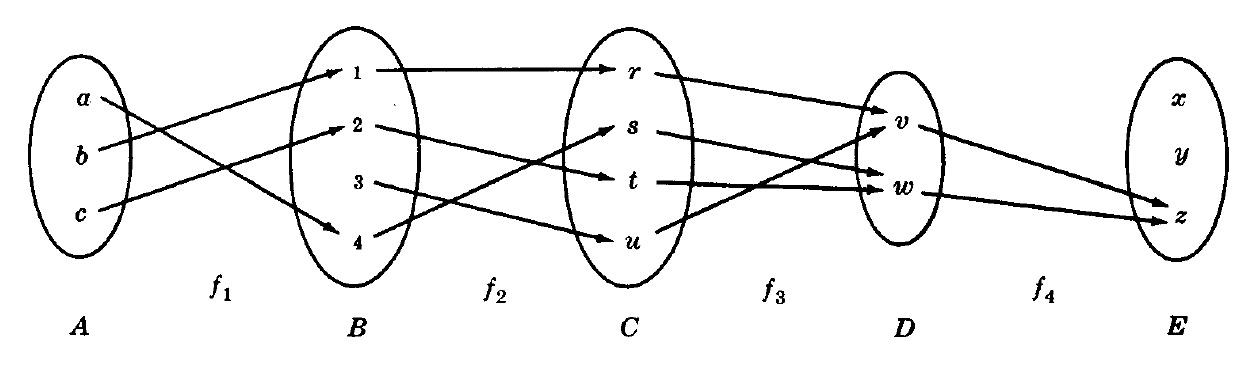
\includegraphics[width=10cm,keepaspectratio=true]{./MD02_IM01.png}
 % MD02_IM01.png: 0x0 pixel, 300dpi, 0.00x0.00 cm, bb=
 \label{fig:MD0201}
\end{figure}

\end{exmp}

\end{frame}

\begin{comment}
\subsubsection{Como encontrar funciones inversas}

\begin{frame}
 Si $f:A \to B$ no es \emph{sobre,} es decir, $f(A) \subset B$ pero $f(A)\neq B,$ basta restringir su codominio a la imagen $f(A)$ para que se convierta en {sobre}:
 $$
 f: A \to f(A).
 $$
\end{frame}

\begin{frame}
 \begin{exmp}
  La funci\'on $f:\R \to \R, x \mapsto x^{2}$ no es sobre, pero como 
  $$f(A)=\set{x^2\mid x\in\R}=\set{y\in \R \mid y\geq 0}$$
  la funci\'on $f: \R\to \set{y \geq 0}, x \mapsto x^{2}$ s\'i lo es.
 \end{exmp}

\end{frame}

\begin{frame}
\begin{figure}[h!]
 \centering
 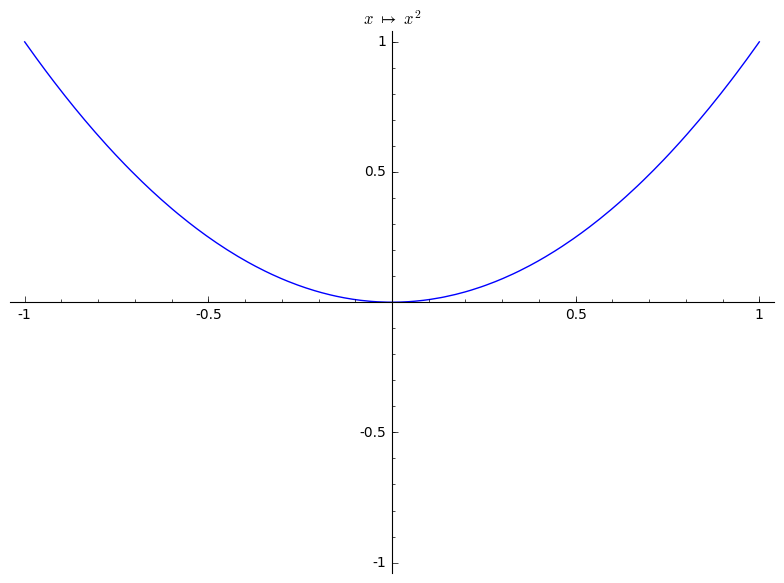
\includegraphics[width=8cm,keepaspectratio=true]{./IMG-04_resticcion.png}
 % IMG-04_resticcion.png: 0x0 pixel, 300dpi, 0.00x0.00 cm, bb=
 \caption{Gráfica de $x^2$}
 \label{fig:0401}
\end{figure}

\end{frame}

\begin{frame}
\begin{prop}
 Si una funci\'on $f:A \to B$ es inyectiva, entonces
 $$
 f:A \to f(A)
 $$ es invertible.
\end{prop}

\end{frame}

\begin{frame}{Como encontrar la inversa de $y=f(x)$}
\begin{enumerate}[(a)]
 \item Verifique que $f(x)$ es un funci\'on $1:1.$ \pause
 \item Despeje la variable independiente $y$ en la ecuaci\'on $y=f(x)$ para obtener
 $$x=f^{-1}(y).$$ \pause
 \item Reescriba la ecuaci\'on anterior intercambiando las variables: $y=f^{-1}(x).$
\end{enumerate}

\end{frame}

\begin{frame}
\begin{exmp}
 Encuentre la inversa de la funci\'on $f(x)=3x-2,$
\end{exmp}

\end{frame}

\begin{frame}
\begin{exmp}
 Encuentre la inversa de $f(x)=\dfrac{x^{5}-3}{2}.$
\end{exmp}

\end{frame}

\begin{frame}
 \begin{exmp}
  Encuentre la inversa de $f(x)=\sqrt{x-2}.$
 \end{exmp}

\end{frame}

\begin{frame}
\begin{figure}[h!]
 \centering
 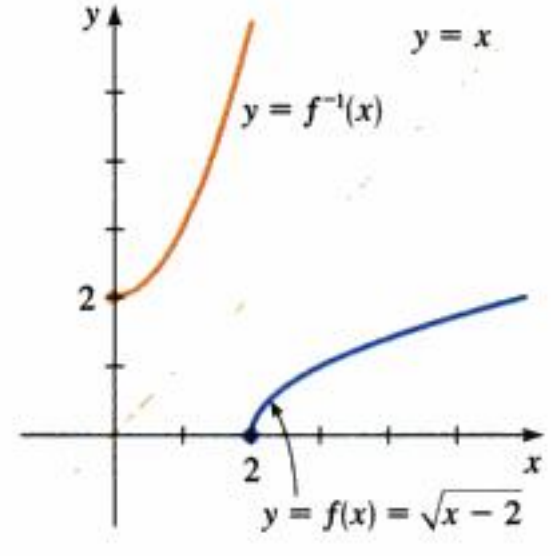
\includegraphics[height=8cm,keepaspectratio=true]{./MD02_sqrt_x-2.png}
 % MD02_sqrt_x-2.png: 0x0 pixel, 300dpi, 0.00x0.00 cm, bb=
 \label{fig:MD02_sqrt_x-2}
\end{figure}

\end{frame}
%\begin{comment}
\subsubsection{Caracterizaci\'on geom\'etrica}

\begin{frame}
Consiere ahora una funci\'on $f:\R \to \R.$ Representemos su gr\'afica 
$$
\Gamma_{f}=\set{(x,y)\in\R^{2}\mid y=f(x)}
=\set{(x,f(x))}
$$
en el plano.
\end{frame}


\begin{frame}
\begin{rem}
 \begin{itemize}
  \item $f:\R \to \R$ es \emph{$1:1$} si cada l\'inea \emph{horizontal} intersecta la gr\'afica de $f$ a lo m\'as en un punto.
  \item $f:\R \to \R$ es \emph{sobre} si cada l\'inea horizontal intersecta la gr\'afica de $f$ al menos en un punto.
  \item $f:\R \to \R$ es \emph{invertible} si cada l\'inea horizontal intersecta la gr\'afica de $f$...
 \end{itemize}

\end{rem}
\end{frame}

\begin{frame}
\begin{exmp}
 Considere las siguientes funciones $:\R \to \R$
 \begin{enumerate}
  \item $x \mapsto x^{2}$
  \item $x \mapsto 2^{x}$
  \item $x \mapsto x^{3}-2x^{2}-5x+6$
  \item $x \mapsto x^{3}$
 \end{enumerate}
y determine si son $1:1,$ sobre o invertibles.
\end{exmp}

\end{frame}

\begin{frame}
\begin{figure}[h!]
 \centering
 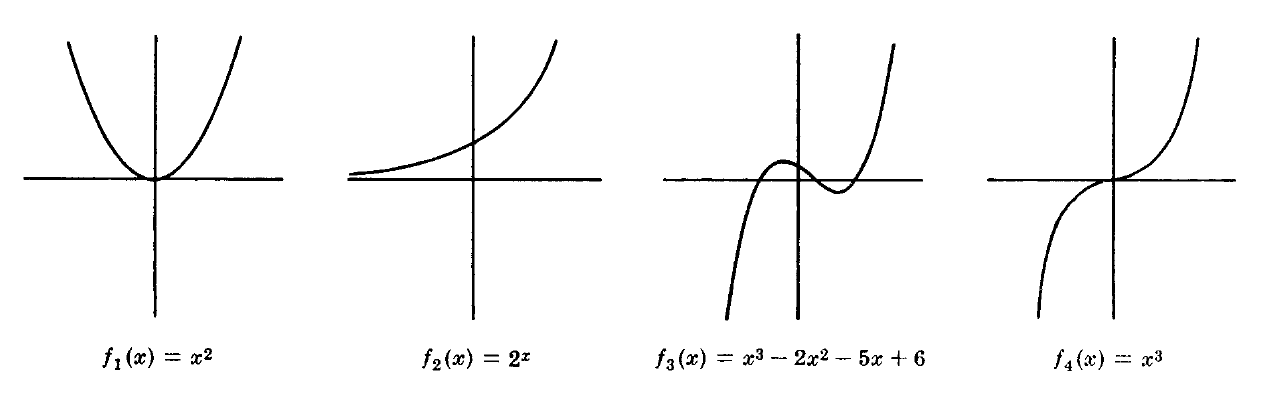
\includegraphics[width=10cm]{./MD02_IM02.png}
 % MD02_IM02.png: 0x0 pixel, 300dpi, 0.00x0.00 cm, bb=
 \label{fig:MD0202}
\end{figure}

\end{frame}

\subsubsection{Permutaciones}

\begin{frame}
Consideremos un conjunto finito $X=\set{x_{1},...,x_{N}},$ esto es, $X$ tiene \emph{cardinalidad} $n(X)=N < \infty.$
\pause

Una funci\'on biyectiva (invertible) $\sigma:X \to X$ es llamada \emph{permutaci\'on} en $X.$
\pause

Observe que las composiciones e inversas de permutaciones, as\'i como la identidad, son tambi\'en permutaciones.
\pause

En este caso, diremos que la permutaci\'on $\sigma$ \emph{actua} en $X.$
\end{frame}

\begin{frame}
Supongamos que la permutaci\'on $\sigma$ actua en $X={x_{1},x_{2},x_{3}}$ de la siguiente manera:
$$
\sigma(x_{1})=x_{2}, \; \sigma(x_{2})=x_{3}, \; \sigma(x_{3})=x_{1}.
$$

Entonces, podemos representar la permitaci\'on de la siguiente manera
$$\sigma=
\begin{pmatrix}
1 & 2 & 3 \\
2 & 3 & 1,
\end{pmatrix},
$$ \pause es decir, s\'olo nos fijamos de que manera actua en el \'indice $j$ del elemento $x_{j}.$
\end{frame}

\begin{frame}
 De manera general, numerando los elemenos de $X=\set{x_{1},...,x_{N}},$ podemos identificar este conjunto con $A_{N}=\set{1,...,N}$ por medio de la biyecci\'on $x_{i} \mapsto i.$
 \pause
 
 Ahora, consideremos una permutaci\'on $\sigma:A_{N}\to A_{N},$ tal que $\sigma(i)=\sigma_{i}.$ Entonces podemos representa $\sigma$ por medio de 
 $$\sigma=
 \begin{pmatrix}
  1& ... & N \\
  \sigma_{1}& ... & \sigma_{N}.
 \end{pmatrix}
$$
\pause

El conjunto de todas las permutaciones $:A_{N}\to A_{N}$ se denota por $S_{N}$ y tiene una cardinalidad 
$n(S_{N})=N!.$
\end{frame}
\end{comment}
\end{document}
